\documentclass{article}
\usepackage{neb-macros}

\usepackage{tikz}
\usetikzlibrary{calc,intersections,through,backgrounds}

\begin{document}

\CheapTitle{Angles}

\begin{dfn}[Angle]
Let $\mathcal{P}$ be an ordered geometry and $x$, $o$, and $y$ distinct points.
\begin{itemize}
\item The set \[ \Angle{x}{o}{y} = \Ray{o}{x} \cup \Ray{o}{y} \] is called the \emph{angle} with \emph{vertex} $o$ and \emph{sides} $\Ray{o}{x}$ and $\Ray{o}{y}$.
\item Suppose further that $x$, $o$, and $y$ are not collinear. In this case, since $\mathcal{P}$ is an ordered geometry, the lines $\Line{o}{x}$ and $\Line{o}{y}$ divide $\mathcal{P}$ into half-planes. Let $H_1$ be the $y$ half-plane of $\Line{o}{x}$, and let $K_1$ be the $x$ half-plane of $\Line{o}{y}$. We define the \emph{interior} of $\Angle{x}{o}{y}$ to be the set \[ \IntAngle{x}{o}{y} = H_1 \cap K_1. \] If $x$, $y$, and $o$ are collinear, then the interior of $\Angle{x}{o}{y}$ is not defined.
\end{itemize}
\end{dfn}



\begin{dfn}[Linear Pair, Vertial Pair]
Suppose $x$, $y$, $z$, $w$, and $o$ are distinct points in an ordered geometry.
\begin{itemize}
\item $\Angle{x}{o}{y}$ and $\Angle{y}{o}{z}$ are called an \emph{adjacent pair} if $y \in \IntAngle{x}{o}{z}$.
\item $\Angle{x}{o}{y}$ and $\Angle{y}{o}{z}$ are called a \emph{linear pair} if $\Between{x}{o}{z}$.
\item $\Angle{x}{o}{y}$ and $\Angle{z}{o}{w}$ are called a \emph{vertical pair} if $\Between{x}{o}{z}$ and $\Between{y}{o}{w}$.
\end{itemize}
\end{dfn}

\begin{thm}[Crossbar Theorem]
Suppose $O$, $A$, and $B$ are noncollinear points in an ordered geometry, and that $C \in \IntAngle{A}{O}{B}$. Then $\Ray{O}{C}$ cuts $\Segment{A}{B}$ at a unique point $D$.
\end{thm}

\begin{center}
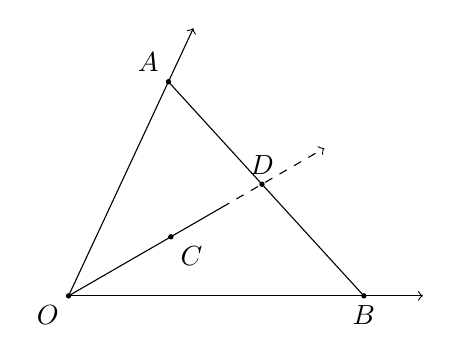
\begin{tikzpicture}[scale=1.5]
  \coordinate [label=below left:$O$] (O)   at (0  : 0);
  \coordinate [label=above left:$A$] (A)   at (65 : 2);
  \coordinate (A')  at (65 : 2.5);
  \coordinate [label=below:$B$]      (B)   at (0  : 2.5);
  \coordinate (B')  at (0  : 3);
  \coordinate (C)   at (30 : 1);
  \coordinate (C')  at (30 : 1.5);
  \coordinate (C'') at (30 : 2.5);

  \coordinate [label=above:$D$]      (D)   at (intersection of A--B and O--C'');

  \draw [->] (O) -- (A');
  \draw [->] (O) -- (B');

  \draw [fill] (O) circle [radius=0.5pt];
  \draw [fill] (A) circle [radius=0.5pt];
  \draw [fill] (B) circle [radius=0.5pt];

  \draw (O) -- (C');
  \draw [dashed, ->] (C') -- (C'');

  \draw [fill] (C) circle [radius=0.5pt];
  \node [below right] at (C) {$C$};

  \draw (A) -- (B);

  \draw [fill] (D) circle [radius=0.5pt];
\end{tikzpicture}
\end{center}

\begin{proof}
By the Interpolation property, there is a point $P$ on $\Line{O}{A}$ such that $\Between{P}{O}{A}$. Note that $A$ and $P$ are on opposite sides of $\Line{O}{B}$, so that $P$ and $C$ are on opposite sides of $\Line{O}{B}$. (Since $A$ and $C$ are on the same side of $\Line{O}{B}$ by definition.) Consider now the triangle $\Triangle{P}{A}{B}$. Note that the line $\Line{O}{C}$ does not contain $A$, $B$, or $P$, since $C$ is not on $\Line{O}{A}$ or $\Line{O}{B}$ by hypothesis. Moreover, $\Line{O}{C}$ cuts $\Segment{P}{A}$ at $O$. By Pasch's Axiom, $\Line{O}{C}$ must also cut either $\Segment{P}{B}$ or $\Segment{A}{B}$.

Suppose $\Line{O}{C}$ cuts $\Segment{P}{B}$ at a (necessarily unique) point $Q$. Note that $\Line{O}{C} = \Line{Q}{C}$. Now $P$ and $Q$ are on the same side of $\Line{O}{B}$, so that $Q$ and $C$ are on \emph{opposite} sides of $\Line{O}{B}$. Thus, there is a unique point $R$ on $\Line{O}{B}$ such that $\Between{Q}{R}{C}$. In particular, $R \in \Line{O}{C}$. Now we have $O,R \in \Line{O}{C}$ and $O, R \in \Line{O}{B}$, so that $\Line{O}{C} = \Line{O}{B}$, a contradiction.

Hence $\Line{O}{C}$ must cut $\Segment{A}{B}$ at a unique point; say $D$. Now $D$ and $A$ are on the same side of $\Line{O}{B}$, and so $C$ and $D$ are on the same side of $\Line{O}{B}$; in particular, we cannot have $\Between{D}{O}{C}$. So in fact $\Ray{O}{C}$ cuts $\Segment{A}{B}$ at a unique point.
\end{proof}

\end{document}
